\documentclass{beamer}
\usepackage{amsmath}
\usepackage{amssymb}
\usepackage[utf8]{inputenc}
\usepackage[ngerman]{babel}
\usepackage{lastpage}
\usepackage{listings}
\usepackage{caption}
\usepackage{color}
\usepackage{fancyvrb}
\usepackage{url}
\usepackage{xcolor}

\usepackage{tikz}
\usetikzlibrary{positioning, shapes}
\usetikzlibrary{arrows}

%Für [Seite]/[Anzahl-Seiten] in der unteren rechten ecke
\newcommand*\oldmacro{}%
\let\oldmacro\insertshorttitle%
\renewcommand*\insertshorttitle
{
	\oldmacro\hfill%
	\thepage\,/\,\pageref{LastPage}
}
\makeatletter
\newcommand*{\currentname}{\TR@currentTitle}
\makeatother

\definecolor{light-light-gray}{gray}{0.85}

\usetheme[compress]{Berlin}
\setbeamerfont{headline}{size=\large}
\setbeamerfont*{section in head/foot}{size=\tiny}
\setbeamertemplate{toc}{circle}
\setbeamertemplate{itemize subitem}[triangle] % if you want a triangle
\setbeamercovered{transparent}
%%\usetheme[compress]{Berlin}
%\usetheme[compress]{Dresden}
%%\usetheme{Hamburg}
%\setbeamerfont{headline}{size=\large}
%\setbeamerfont*{section in head/foot}{size=\tiny}
%\setbeamercovered{transparent}
%\setbeamertemplate{bibliography item}[text]
%\setbeamertemplate{itemize items}[square]
%\setbeamertemplate{itemize subitem}[triangle]
%\setbeamertemplate{section in toc}[square]
%\setbeamertemplate{subsection in toc}[square]
%\setbeamertemplate{caption}[numbered]
%\setbeamercolor*{title}{use=structure,fg=white,bg=structure.fg}
%\setbeamertemplate{title page}[default][colsep=-2bp]
%\setbeamercolor{block title}{bg=darkred2!100,fg=white}
%\setbeamercolor{block body}{bg=darkred3!25,fg=black}

\definecolor{myBlue}{rgb}{0,0.55,0.8}
%\definecolor{darkred2}{rgb}{0,0.41,0.6}
%\definecolor{darkred3}{rgb}{0.2,0.4,0.6}
\usecolortheme[named=myBlue]{structure}

\title{IP over Avian Carriers (IPoAC)}
\subtitle{\small Rettet die Bäume}%Und was es mit dem Fällen von Bäumen zu tun hat.}
\author{by \href{http://hauke-stieler.de/}{Hauke Stieler}\vspace{-6ex}}
\date{\vspace{50pt}\href{http://hauke-stieler.de/}{\scriptsize{4stieler}}\\\vspace{-30pt}\today}
%\titlegraphic{\href{http://uni-hamburg.de/}{\includegraphics[height=.15\textheight]{./images/logo}}}

\begin{document}
	\begin{frame}
		\maketitle
	\end{frame}
	\begin{frame}
		\tableofcontents[hideallsubsections]
	\end{frame}
	\section{Internet bisher}
	\subsection{Aufbau}
	\begin{frame}
		\begin{columns}
			\begin{column}{0.5\textwidth}
				\begin{itemize}
					\item Hardware (harter Stoff)
					\begin{itemize}
						\item Kabel, etc.
					\end{itemize}\pause
					\item Network (Nettoarbeit)
					\begin{itemize}
						\item Ethernet, ISDN, DSL
						\item IP(-Adressen)
						\item TCP, UDP
					\end{itemize}\pause
					\item Software (weiches Zeugs)
					\begin{itemize}
						\item HTTP(s), FTP, DNS, SMTP, ...
					\end{itemize}
				\end{itemize}
			\end{column}
			\begin{column}{0.4\textwidth}
				\begin{figure}[ht]
					\href{https://c1.staticflickr.com/1/84/231641275_17c37e3601.jpg\# this-image-is-creative-commons}{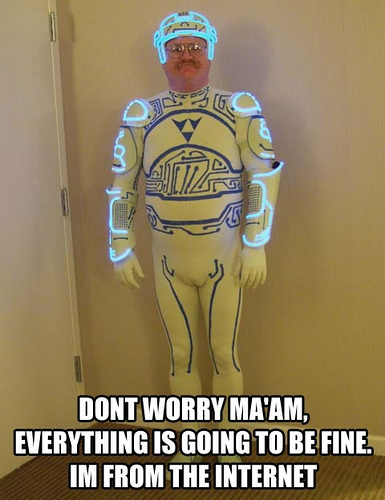
\includegraphics[width=\textwidth,height=0.65\textheight,keepaspectratio]{./images/im-from-the-internet}}
				\end{figure}
			\end{column}
		\end{columns}
	\end{frame}
	\subsection{Pakete}
	\begin{frame}
		\footnotesize
		\begin{tabular}{|c|c|c|c|c|}
			\hline
			header & IP-header & TCP-header & data & chksm\\
			14 bytes & 20 bytes & 20 bytes & \hspace{30pt}1460 bytes\hspace{30pt} & 2 bytes\\
			\hline
		\end{tabular}\\\vspace{1cm}
	\end{frame}
	\subsection{Übertragung}
	\begin{frame}
	\begin{tikzpicture}[->,>=stealth,shorten <= 3pt,shorten >= 3pt]

		\node[ellipse,draw](user1) at (0, 0) {\footnotesize User};
		\node[cloud, cloud puffs=12, cloud ignores aspect, minimum width=3.5cm, minimum height=2cm, align=center, draw] (cloud) at (3.75, 0) {\footnotesize Internetz};
		\node[ellipse,draw,text width=2.2cm] (user2) at (8.5, 0) {\footnotesize ...other User\vspace{-5pt} \tiny{who else?}};
		
		\path[line width=0.75pt] (user1) edge node {} (cloud);
		\path[line width=0.75pt] (cloud) edge node {} (user2);

	\end{tikzpicture}
	\end{frame}
	\subsection{Nachteile}
	\begin{frame}
		\begin{columns}
			\begin{column}{0.35\textwidth}
				\begin{itemize}
					\item Langsam 
					\item Doof 
					\item Teuer 
					\item Fehleranfällig 
				\end{itemize}
			\end{column}
			\begin{column}{0.55\textwidth}
				\begin{figure}[ht]	\href{http://fc04.deviantart.net/fs70/f/2013/095/9/f/say_what____internet_speed_meme__by_benchamberlainneo-d60j8sz.png\# this-image-is-creative-commons}{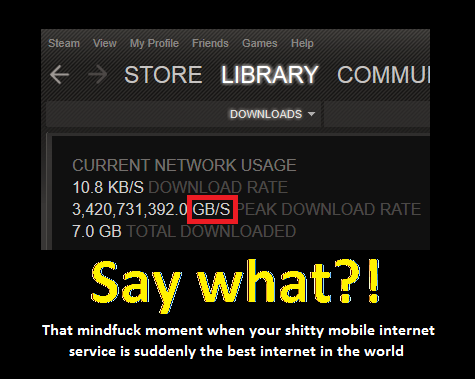
\includegraphics[width=\textwidth,keepaspectratio]{./images/speed}}
				\end{figure}
			\end{column}
		\end{columns}
	\end{frame}
	\section{Allgemeines}
	\subsubsection{RFCs}
	\begin{frame}
		\begin{itemize}
			\item \texttt{RFC 1149} und \texttt{RFC 2549}
			\item \texttt{RFC} $\rightarrow$ \textbf{R}equest \textbf{f}or \textbf{C}omments
			\item RFC-Dokumente sind Vorschläge/Dokumente für Diskussionen
		\end{itemize}
	\end{frame}
	\subsection{Avian Carrier?}
	\begin{frame}
		\begin{itemize}
			\item Verkapselung von \textit{IP-datagrams} in \textit{avian carriers}\\
				$\rightarrow$ \textit{IP over Avian Carrier} (IPoAC)
			\item Nützlich in Ballungsgebieten\\
				$\rightarrow$ MANs (Metropolitan Area Networks) 
			\item Was es bietet? 
			\begin{itemize}
				\item Hohe Verzögerung 
				\item Geringer Durchsatz 
				\item Tiefflug-Service (low altitude service)
			\end{itemize}
		\end{itemize}
	\end{frame}
	\section{Details}
	\subsection{Die Technologie}
	\begin{frame}
		\begin{itemize}
			\item Punkt-zu-Punkt Weg (point-to-point path) für jeden normalen Carriers 
			\item Keine Interferenz zwischen Carriern 
			\item Nahezu \textit{unlimitierte} Carrier-Anzahl\\
				$\rightarrow$ \textit{3D-ether-space technology} (3DEST)\\
				$\rightarrow$ bisher: \textit{1D-ether-space} durch IEEE802.3 
			\item Intrinsische Kollisions Vermeidung\\
				\textit{intrinsic collision avoidance system} (ICAS) 
			\item Keine \textit{line-of-sight} Technologie\\
				$\rightarrow$ mit Hubs möglich
		\end{itemize}
	\end{frame}
	\subsection{Codierungs- und Leseverfahren}
	\begin{frame}
		\begin{itemize}
			\item Codierung als HEX
			\item Oktettweise Trennung
			\item Auftragen auf längliches Stück Papier
			\item Mit duct-tape am Carrier-Bein befestigen
			\item \textit{Maximum Transmission Unit} (MTU) ca. 256\pause  mg
		\end{itemize}
	\end{frame}
	\begin{frame}
		\begin{itemize}
			\item Duct-tape lösen
			\item Informationen optisch scannen
		\end{itemize}
	\end{frame}
	\begin{frame}
		\begin{figure}[ht]	
			\vspace{-1.5cm}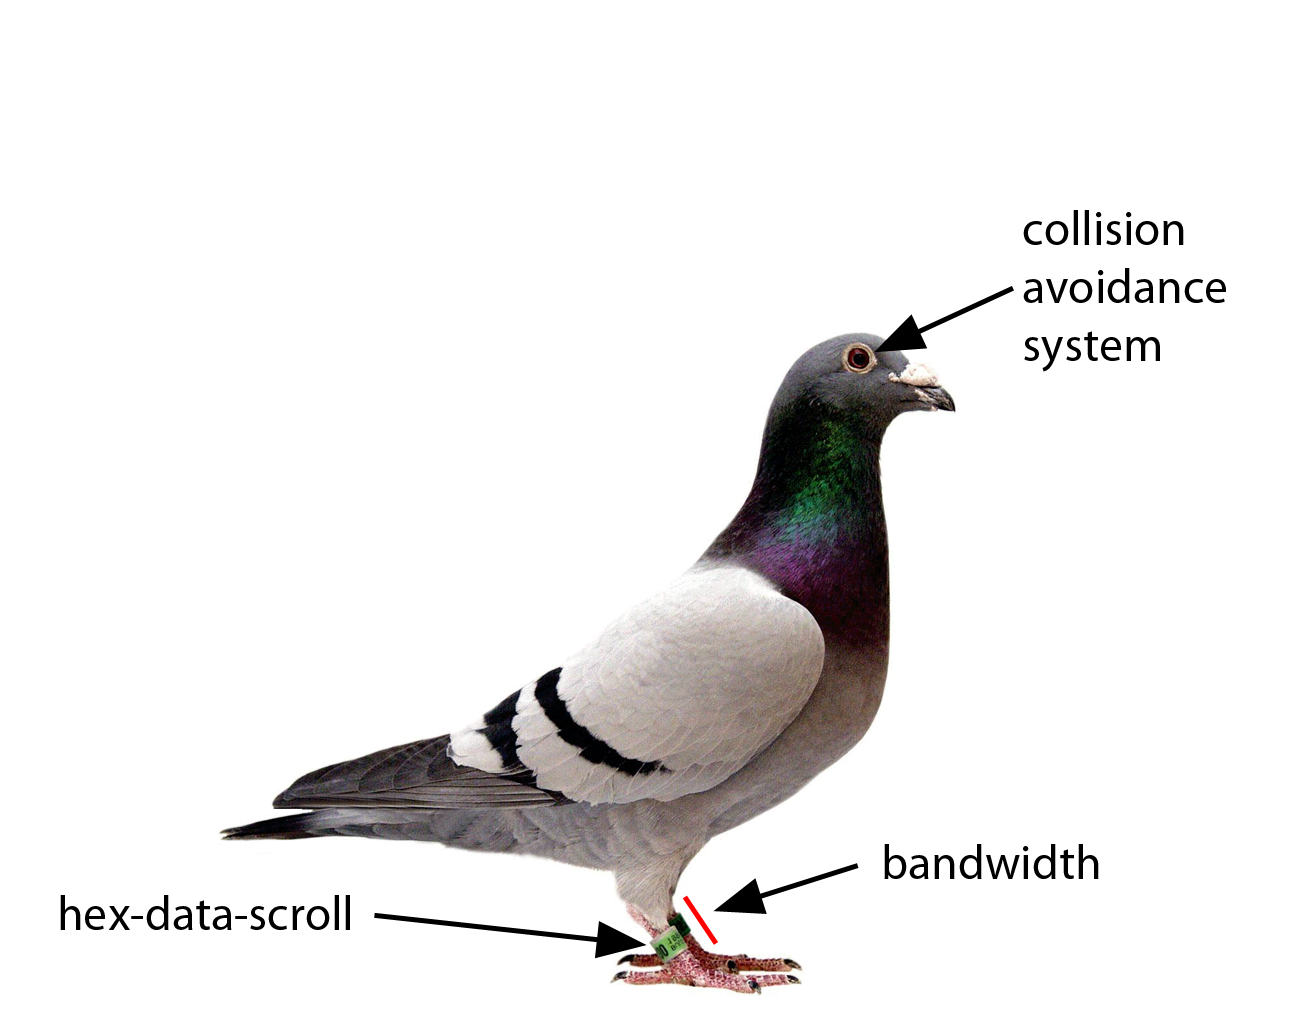
\includegraphics[height= \textheight]{./images/carrier-pic}
		\end{figure}
	\end{frame}
	\subsection{Alternativen}
	\begin{frame}
		\begin{itemize}
			\item \textit{Avian Ostriches Carrier} (AOC)\\
				$\rightarrow$ langsamer\\
				$\rightarrow$ höhere MTU\\
				$\rightarrow$ \textit{domain-bridges} benötigt
			\item \textit{Round-robin queueing} (RRQ)\\
				$\rightarrow$ Leistungsstark\\
				$\rightarrow$ Nicht empfohlen\\
				$\rightarrow$ Keine \textit{auto-homing} Funktion
		\end{itemize}
	\end{frame}
	\subsection{Zu beachten}
	\begin{frame}
		\begin{itemize}
			\item \textit{Network Adress Translations} (NATs) nicht empfohlen\\
				$\rightarrow$ schwierige Änderung der \textit{brain-embedded IP-adresses}\\
				$\rightarrow$ Eventuell isst Carrier den NAT
			\item Keine Frischhaltefolie verwenden!
			\item \textit{Multicasting} möglich $\rightarrow$ \textit{clone-device} benötigt
		\end{itemize}
	\end{frame}
	\begin{frame}
		\begin{itemize}
			\item Carrier verloren, wenn Bäume geschnitten/gefällt werden\\
				$\Rightarrow$ Rettet Bäume für schnelleres Internet
			\item Verbreitung über \textit{inheritance-tree}
			\item TTL bei ca. 15 Jahren
			\item IPv6, bzw. ACv6 möglich
		\end{itemize}
	\end{frame}
	\section{Einsatz}
	\begin{frame}[fragile=singleslide]
	\fontsize{8}{8}\selectfont
	\texttt{vegardgyversalen:~\$ /sbin/ifconfig tun0\\
tun0~~~~~~Link encap:\textcolor{red}{Point-to-Point} Protocol\\
~~~~~~~~~~inet addr:10.0.3.2  P-t-P:10.0.3.1  Mask:255.255.255.255\\
~~~~~~~~~~UP POINTOPOINT RUNNING NOARP MULTICAST  MTU:150  Metric:1\\
~~~~~~~~~~RX packets:1 errors:0 dropped:0 overruns:0 frame:0\\
~~~~~~~~~~TX packets:2 errors:0 dropped:0 overruns:0 carrier:0\\
~~~~~~~~~~\textcolor{red}{collisions:0}\\
~~~~~~~~~~RX bytes:88 (88.0 b)  TX bytes:168 (168.0 b)\\\hfill\\
vegardgyversalen:~\$ ping -c 9 -i 900 10.0.3.1\\
PING 10.0.3.1 (10.0.3.1): 56 data bytes\\
64 bytes from 10.0.3.1: icmp\_seq=0 ttl=255 time=6165731.1 ms\\
64 bytes from 10.0.3.1: icmp\_seq=4 ttl=255 time=3211900.8 ms\\
64 bytes from 10.0.3.1: icmp\_seq=2 ttl=255 time=5124922.8 ms\\
64 bytes from 10.0.3.1: icmp\_seq=1 ttl=255 time=6388671.9 ms\\\hfill\\
--- 10.0.3.1 ping statistics ---\\
9 packets transmitted, 4 packets received, 55\% packet loss\\
round-trip min/avg/max = 3211900.8/\textcolor{red}{5222806.6}/6388671.9 ms
}\normalsize\\
	\begin{itemize}
		\item \texttt{avg = }87 Minuten
		\item bis 0.08 bytes-per-second (bps) möglich
	\end{itemize}
	\end{frame}
	\section*{Next time ...}
	\begin{frame}
		\begin{center}
			\textbf{\underline{Nächstes mal:}}\\\hfill\\
			Peer-to-peer Netzwerk mit Hilfe von Turnschuhen
		\end{center}
	\end{frame}
\end{document}